% =====================================================================================
% Sec. 4  Selection and confidence (C1).  Owner: abhiraj.  FALLBACK skeleton by ojas
% (branch ojas/paper-c1): abhiraj may rewrite any of it; his draft wins.
%
% NO RESULTS EXIST YET.  Every number is a macro from paper/tables/c1/macros_c1.tex (written
% by scripts/c1_paper_outputs.py from the report-half results; main.tex \inputs it when it
% exists), or a design macro (\Viva...) of documents/viva-slides/macros_setup.tex.  Result
% macros are called through \Cres{<name>} / \CresCI{<name>}, which print a bold ? while the
% macro is undefined, so the paper builds before the results land.
%
% Slots:  % TODO(results): ...   wording that depends on a sign or a decision; both (or all)
%                                phrasings are written out; keep one, delete the rest.
%         % TODO(outputs): ...   a number the paper wants that c1_paper_outputs.py does not
%                                write as a macro yet.  None open: the three slots of the
%                                first draft (shared-error term and ICC; gamma_2..4 and their
%                                Holm; additive calibrator) are wired to the PR #31 macros.
%
% Worked examples use LLaDA-8B-Base, uniform states (the script's default main arm and the
% arm of fig:c1-delta); swap to another arm by changing the label in the names.
% Macro name pattern (per-arm files, scripts/analyze_traces.py):
%   COne<Label>{Gap<m>,Field<m>,Own<m>,Contrast,ECE,BetaZNoFE,BetaZFE}<Tag>[Lo|Hi]
%   <Tag> = Uni | DecTopkConfKFour | UniMatchedTopkConfKFour ...;  <m> = One ... ThirtyTwo
%   COneFieldContrast<Label><Tag>[Lo|Hi], COneHolmDecision{EOne,ETwo}<Label><Tag>,
%   COne{HolmEOneFamily,HolmEOneReject,DeclaredEOne,ConfirmedEOne} (and ETwo)  macros_c1.tex
%   COne<Label>Residual<m><Tag>[Lo|Hi], COne<Label>ICC<Tag>[Lo|Hi]               macros_c1.tex
%   COne<Label>Gamma{Two,Three,Four}<Tag>[Lo|Hi], COneHolmPGamma<k><Label><Tag>,
%   COneHolmGamma{Family,Reject,Rows}                                              macros_c1.tex
%   COneFieldContrast<Label>{KnotsFive,KnotsThirteen,Clean,Additive}<Tag>[Lo|Hi],
%   COneFieldAdditive{Shift,Agree}<Label><Tag>, COneAdditive{Runs,Cells,Agree}      macros_c1.tex
%   COneHolmFootnote (the starred-table note; HolmM, HolmMissing[Count] inside it)
%   EThree<Label>TypeEffectTopkConfK<k>{Matched,Grid}[Lo|Hi], ...TypeTestP...       e3
%   TEight<Label>{Position,TokenType,TemperatureLogodds}{EOne,ETwo}<Tag>{Without,With,
%   Difference}[Lo|Hi];  TEightLladaBasePrecisionPrecision{EOne,ETwo}<Tag>...      t8
%
% Labels defined here: sec:c1, sec:c1-main, sec:c1-beta, sec:c1-e3, sec:c1-t8,
% sec:c1-robust, tab:c1-main, fig:c1-delta; in appendix_c1.tex: sec:c1-app, tab:c1-e3,
% tab:c1-t8, tab:c1-sens, tab:c1-gamma, tab:c1-shared (and tab:c1-beta, commented out there for space).  Used from Secs. 2-3: sec:setup, eq:gap, prop:select, prop:split,
% eq:gapsplit, sec:instrument, tab:runs, sec:traces, sec:estimands, eq:eqtwo, eq:eqthree,
% sec:inference, sec:validation, sec:prereg.
% Needs booktabs (the generated tables) and graphicx.
% =====================================================================================

\providecommand{\Cres}[1]{\ifcsname #1\endcsname\csname #1\endcsname\else\textbf{?}\fi}
\providecommand{\CresCI}[1]{\ensuremath{\Cres{#1}\;[\Cres{#1Lo},\,\Cres{#1Hi}]}}
% \Cfit{<table>}: the table at its natural width, shrunk to the line only if it is wider.
\ifdefined\Cfitbox\else\newsavebox{\Cfitbox}\fi
\providecommand{\Cfit}[1]{\sbox{\Cfitbox}{#1}%
  \ifdim\wd\Cfitbox>\linewidth\resizebox{\linewidth}{!}{\usebox{\Cfitbox}}\else\usebox{\Cfitbox}\fi}
% \Cpending{<what>}: the box a generated table or figure is replaced by until it exists.
\providecommand{\Cpending}[1]{\fbox{\parbox{0.9\linewidth}{\centering\small #1: pending results
  (\texttt{scripts/c1\_paper\_outputs.py})}}}

\section{Selection and confidence (C1)}
\label{sec:c1}

C1 asks whether a committed token's confidence overstates its accuracy more when it won a
larger field, and how much of that is the field term of Proposition~\ref{prop:split}. Every
number is from the report half, computed by the frozen commands (\S\ref{sec:prereg}).

\paragraph{Arms and claims.}
The seven arms at the top of Table~\ref{tab:runs} are analysed in uniform states and in those
of the teacher-forced top-$k$ decoder at $k=4$ (\S\ref{sec:traces}). The E1 contrast
$\Delta(\VivaPoolMax)-\Delta(1)$ and the E2 contrast field$(\VivaPoolMax)-$field$(1)$ each form one
Holm family over these 14 cells, and $\gamma_2,\gamma_3,\gamma_4$ of Eq.~\ref{eq:eqthree} one
within each arm (\S\ref{sec:inference}).
% Claim rule: prereg/frozen_config.json settled.claim_rule (PR #19, deviations.md 16c,d);
% alpha 0.05, family size 14, a missing member counts as p = 1.
We claim an E1 or E2 effect only if it is declared, its 95\% interval excluding 0, \emph{and}
Holm rejects it at $\alpha=0.05$ within its family ($m=14$; a missing cell counts as $p=1$).
Everything else is exploratory, reported with its interval and no claim: decoder states at
$k\in\{2,8\}$, matched uniform states, $\beta_z$, $\gamma_k$, E3, T8, and the clean, time-split,
additive-calibrator and knot runs (200 resamples; descriptive intervals).

% ------------------------------------------------------------------- floats
\begin{table*}[t]
  \centering
  \IfFileExists{tables/c1/c1_main.tex}{\Cfit{% Generated by scripts/c1_paper_outputs.py from results/c1/<Label>/results.json, results/c1/summary/c1_summary.json -- do not edit by hand.
% Needs booktabs.  --- is an em dash: the arm or variant is not in the results.
\begingroup\footnotesize\setlength{\tabcolsep}{2.5pt}
\begin{tabular}{lllclcll}
\toprule
Arm & Masks & E1 & Holm & E2 & Holm & $\beta_z$ & $\beta_z^{\mathrm{FE}}$ \\
\midrule
LLaDA Base & uniform & $-0.003$$^{*,\dagger}$ {\scriptsize[$-0.004$, $-0.002$]} & yes & $0.001$$^{*,\dagger}$ {\scriptsize[$0.001$, $0.001$]} & yes & --- & --- \\
 & dec. $k{=}4$ & $0.006$$^{*,\dagger}$ {\scriptsize[$0.005$, $0.008$]} & yes & $0.004$$^{*,\dagger}$ {\scriptsize[$0.004$, $0.004$]} & yes & --- & --- \\
\addlinespace
Dream Base & uniform & $-0.002$$^{*,\dagger}$ {\scriptsize[$-0.004$, $-0.001$]} & yes & $0.001$$^{*,\dagger}$ {\scriptsize[$0.001$, $0.001$]} & yes & --- & --- \\
 & dec. $k{=}4$ & $0.015$$^{*,\dagger}$ {\scriptsize[$0.013$, $0.017$]} & yes & $0.003$$^{*,\dagger}$ {\scriptsize[$0.003$, $0.003$]} & yes & --- & --- \\
\addlinespace
LLaDA-I GSM8K & uniform & $-0.022$$^{*,\dagger}$ {\scriptsize[$-0.025$, $-0.018$]} & yes & $-0.003$$^{*,\dagger}$ {\scriptsize[$-0.004$, $-0.003$]} & yes & --- & --- \\
 & dec. $k{=}4$ & $0.024$$^{*,\dagger}$ {\scriptsize[$0.016$, $0.032$]} & yes & $0.021$$^{*,\dagger}$ {\scriptsize[$0.020$, $0.023$]} & yes & --- & --- \\
\addlinespace
LLaDA-I MBPP & uniform & $0.025$$^{\dagger}$ {\scriptsize[$0.003$, $0.051$]} & no & $0.013$$^{*,\dagger}$ {\scriptsize[$0.010$, $0.016$]} & yes & --- & --- \\
 & dec. $k{=}4$ & $0.156$$^{*,\dagger}$ {\scriptsize[$0.126$, $0.189$]} & yes & $0.036$$^{*,\dagger}$ {\scriptsize[$0.031$, $0.041$]} & yes & --- & --- \\
\addlinespace
Dream-I GSM8K & uniform & $0.061$$^{*,\dagger}$ {\scriptsize[$0.052$, $0.070$]} & yes & $0.021$$^{*,\dagger}$ {\scriptsize[$0.020$, $0.023$]} & yes & --- & --- \\
 & dec. $k{=}4$ & $0.072$$^{*,\dagger}$ {\scriptsize[$0.064$, $0.081$]} & yes & $0.038$$^{*,\dagger}$ {\scriptsize[$0.036$, $0.039$]} & yes & --- & --- \\
\addlinespace
Dream-I MBPP & uniform & $0.257$$^{*,\dagger}$ {\scriptsize[$0.227$, $0.290$]} & yes & $0.176$$^{*,\dagger}$ {\scriptsize[$0.159$, $0.194$]} & yes & --- & --- \\
 & dec. $k{=}4$ & $0.186$$^{*,\dagger}$ {\scriptsize[$0.151$, $0.224$]} & yes & $0.076$$^{*,\dagger}$ {\scriptsize[$0.066$, $0.086$]} & yes & --- & --- \\
\addlinespace
MDLM-110M & uniform & $0.002$$^{\dagger}$ {\scriptsize[$0.000$, $0.003$]} & no & $0.002$$^{*,\dagger}$ {\scriptsize[$0.002$, $0.002$]} & yes & --- & --- \\
 & dec. $k{=}4$ & $0.009$$^{*,\dagger}$ {\scriptsize[$0.007$, $0.011$]} & yes & $-0.002$$^{*,\dagger}$ {\scriptsize[$-0.002$, $-0.002$]} & yes & --- & --- \\
\bottomrule
\end{tabular}
\endgroup
% * = claimed: declared (dagger) and rejected by Holm in its family; the family size and
% any missing member are in \COneHolmFootnote (macros_c1.tex).  Holm column: the decision
% of the Holm step alone (yes / no; expl. = exploratory arm, outside the families).
}}{\Cpending{C1 main table}}
  \caption{C1 primary endpoints. E1 $=\Delta(\VivaPoolMax)-\Delta(1)$ and E2 $=$
    field$(\VivaPoolMax)-$field$(1)$, with 95\% intervals (\VivaNBoot{} document resamples).
    Holm: decision of the Holm step. $^\dagger$declared; $^*$claimed. $\beta_z$,
    $\beta_z^{\mathrm{FE}}$: Eq.~\ref{eq:eqtwo} without and with state fixed effects
    ($^\ddagger$interval excludes 0; $^\S$no convergence). TS: time-split set, outside the
    families. ---: absent.}
  \label{tab:c1-main}
  \par\smallskip{\footnotesize\raggedright\Cres{COneHolmFootnote}\par}
\end{table*}

\begin{figure}[t]
  \centering
  \IfFileExists{figures/c1/c1_delta_m_LladaBase.pdf}%
    {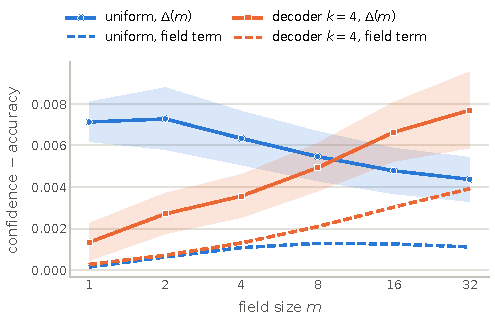
\includegraphics[width=\columnwidth]{figures/c1/c1_delta_m_LladaBase}}%
    {\Cpending{Figure $\Delta(m)$, LLaDA-8B-Base}}
  \caption{LLaDA-8B-Base: $\Delta(m)$ (solid, 95\% band) and its field term (dashed)
    against field size $m$. Solid minus dashed is own miscalibration (Eq.~\ref{eq:gapsplit}).}
  \label{fig:c1-delta}
\end{figure}

% ------------------------------------------------------------------- E1 / E2
\subsection{Does the gap grow with the field?}
\label{sec:c1-main}

Table~\ref{tab:c1-main} gives both contrasts for every arm. Of the
\Cres{COneHolmEOneFamily} E1 tests, Holm rejects \Cres{COneHolmEOneReject} and
\Cres{COneDeclaredEOne} are declared; \Cres{COneConfirmedEOne} meet both and are claims.
For E2 the counts are \Cres{COneHolmETwoReject}, \Cres{COneDeclaredETwo} and
\Cres{COneConfirmedETwo}.
% TODO(results): keep the sentence that matches COneConfirmedEOne and the signs in tab:c1-main.
%   if COneConfirmedEOne > 0 and those contrasts are positive:
%     "In these cells a token that wins a field of 32 is more overconfident than a random
%      masked position: the gap grows with the field. Whether that is a winner's curse is
%      the question of the field term below."
%   if COneConfirmedEOne > 0 and those contrasts are negative:
%     "In these cells the gap shrinks with the field: winners of large fields are less
%      overconfident than a random masked position, the opposite of the winner's curse."
%   if mixed signs: name the runs of each sign; no pooled statement.
%   if COneConfirmedEOne = 0:
%     "No cell meets the claim rule. We find no evidence that the gap changes with field
%      size; the intervals in Table~\ref{tab:c1-main} bound how large a change could be."

For LLaDA-8B-Base in uniform states (Figure~\ref{fig:c1-delta}), $\Delta(1)$, the ordinary
signed calibration error of a masked position, is \CresCI{COneLladaBaseGapOneUni}, beside a
15-bin ECE of $\Cres{COneLladaBaseECEUni}$, and $\Delta(\VivaPoolMax)$ is
\CresCI{COneLladaBaseGapThirtyTwoUni}: E1 is \CresCI{COneLladaBaseContrastUni}. In $k{=}4$
decoder states E1 is \CresCI{COneLladaBaseContrastDecTopkConfKFour}.
% TODO(results): if the decoder and uniform E1 differ in sign or decision for most arms:
%   "The decoder's own states change the picture: <...>." else: "Decoder states give the same
%   picture as uniform ones."  (Row pairs of tab:c1-main.)

\paragraph{How much is the field term?}
At $m=\VivaPoolMax$ the gap splits into own miscalibration
$\Cres{COneLladaBaseOwnThirtyTwoUni}$ and field term $\Cres{COneLladaBaseFieldThirtyTwoUni}$,
and E2 is \CresCI{COneFieldContrastLladaBaseUni}
(decoder states: \CresCI{COneFieldContrastLladaBaseDecTopkConfKFour}).
% TODO(results): if COneConfirmedETwo > 0 (field term grows, E2 > 0):
%   "Part of the growth is the winner's curse proper: at equal confidence, winners of large
%    fields come from contexts where tokens are right less often."
% if E2 is claimed but negative:
%   "The field term falls with m, the opposite of a winner's curse: at equal confidence,
%    winners of large fields come from contexts where tokens are right more often. In
%    simulation a negative field term came from errors shared within a state
%    (sec:validation), which sec:c1-beta checks."
% if COneConfirmedETwo = 0:
%   "The field term does not move with m: whatever change E1 shows is the model's own
%    miscalibration reweighted towards where winners sit, not a winner's curse."
The estimator is not neutral: on simulated traces it read slightly positive when the true
field term was zero (\S\ref{sec:validation}), so a small positive E2 is weaker evidence
than its interval suggests.
The third term of the split, $\E_m[\hat\pi(\ell,s)-a]$, zero without shared errors, is
\CresCI{COneLladaBaseResidualThirtyTwoUni} at $m=\VivaPoolMax$, and the within-state ICC of
residuals is \CresCI{COneLladaBaseICCUni} (Table~\ref{tab:c1-shared}, Appendix).
% TODO(results): if the ICC interval holds 0 and the residual intervals hold 0 in most rows:
%   "Neither shows shared errors: Proposition 1 is a fair description of these states."
% else (ICC > 0 with its interval excluding 0, or a residual excluding 0 at m = 32):
%   "Positions of a state share errors in <arms>; the split has its third term there, and
%    E2 and beta_z are read with that in mind (sec:c1-beta)."
% (m = 1 and the other m: COne<Label>Residual{One,Two,Four,Eight,Sixteen}<Tag>[Lo|Hi].)

% ------------------------------------------------------------------- beta_z
\subsection{The selection diagnostic $\beta_z$}
\label{sec:c1-beta}

$\beta_z$ (Eq.~\ref{eq:eqtwo}) asks the same question by regression: does a winner's rank in
its field predict correctness beyond its own log-odds? Negative without state fixed effects
and near zero with them points to a field effect; nonzero with them, to shared errors
(\S\ref{sec:estimands}). In simulation shared errors gave a \emph{positive} $\beta_z$
without fixed effects and a \emph{negative} field term (\S\ref{sec:validation}), so we read
$\beta_z$ only beside the sign of E2. For LLaDA-8B-Base in uniform states it is
$\Cres{COneLladaBaseBetaZNoFEUni}$ without fixed effects and $\Cres{COneLladaBaseBetaZFEUni}$
with them (Table~\ref{tab:c1-main}).
% TODO(results): keep the reading that matches most arms (count the \ddagger markers in tab:c1-main):
%   (a) beta_z < 0 without FE (CI excludes 0), FE interval holds 0, E2 > 0:
%       "The pattern is that of a field effect, and it agrees with E2."
%   (b) beta_z > 0 without FE and E2 < 0:
%       "The pattern is the one shared errors produced in simulation: positions of a state
%        are wrong together, Proposition 1 does not hold, and E2 is not a field effect."
%   (c) beta_z with FE excludes 0:
%       "Rank predicts correctness within a state, so errors are shared within states and
%        eq:gapsplit gains its third term."
%   (d) every interval holds 0: "beta_z shows no selection effect in either form."
Of the \Cres{COneHolmGammaFamily} tests of $\gamma_2,\gamma_3,\gamma_4$ (Eq.~\ref{eq:eqthree}),
Holm rejects \Cres{COneHolmGammaReject}, in \Cres{COneHolmGammaRows} rows; LLaDA-8B-Base,
uniform: $\gamma_2=\Cres{COneLladaBaseGammaTwoUni}$, $p_{\mathrm{Holm}}=\Cres{COneHolmPGammaTwoLladaBaseUni}$
(Table~\ref{tab:c1-gamma}, Appendix); none is a claim.
% TODO(results): if most rejections are at k = 2 with gamma_2 < 0:
%   "Rank 2 is right less often than rank 1 at equal confidence within a state: the ordering
%    inside a state carries information the confidence does not."  if gamma_2 > 0: "more
%    often: the confidence over-orders the top positions."  if no rejection: "No rank
%    differs from rank 1 once the state is held fixed."  (Unclear sign: name the rows.)

% ------------------------------------------------------------------- E3
\subsection{Decoder states (E3)}
\label{sec:c1-e3}

A decoder visits states whose masked positions are those it was least sure of. E3 asks
whether, at equal confidence and mask rate, tokens in decoder states are right less often
than in uniform states with as many masks (\S\ref{sec:estimands}); the decoder is
teacher-forced, so this is the effect of which positions remain masked, not of its own
mistakes. All E3 rows are exploratory (Table~\ref{tab:c1-e3}, Appendix~\ref{sec:c1-app}). For
LLaDA-8B-Base at $k=4$ the difference, positive if decoder-state tokens are right less
often, is \CresCI{EThreeLladaBaseTypeEffectTopkConfKFourMatched} against matched uniform
states (sup-$t$ $p=\Cres{EThreeLladaBaseTypeTestPTopkConfKFourMatched}$) and
\CresCI{EThreeLladaBaseTypeEffectTopkConfKFourGrid} against the reweighted uniform grid.
% TODO(results): if most matched-uniform rows are positive with intervals excluding 0:
%   "Confidence means less in the states a decoder actually visits: a calibration curve fitted
%    on training-style masks overstates accuracy there, so a calibrator for decoding should
%    be fitted on decoder states (sec:c3)."
% if negative: "Decoder-state tokens are right more often than their confidence suggests
%   relative to uniform states: the decoder's states are, if anything, easier at equal
%   confidence."
% if intervals hold 0 / sup-t p > 0.05 for most rows: "At equal confidence and mask rate,
%   decoder states and uniform states give the same accuracy: the state pattern does not
%   shift calibration."
% Wide figure available: figures/c1/c1_e3_LladaBase.pdf (reliability + difference curve,
% 6.9 in); add as figure* only if space allows.

% ------------------------------------------------------------------- T8
\subsection{Controls (T8)}
\label{sec:c1-t8}

A change of $\Delta$ with $m$ could come from what winners are rather than from winning:
where they sit, what kind of token they are, or a model over- or underconfident by mask
rate. Each control removes one (\S\ref{sec:estimands}); Table~\ref{tab:c1-t8}
(Appendix~\ref{sec:c1-app}) gives E1 and E2 without and with it and the paired difference. For LLaDA-8B-Base in uniform states the change in E1 is
\CresCI{TEightLladaBasePositionEOneUniDifference} for position,
\CresCI{TEightLladaBaseTokenTypeEOneUniDifference} for token type and
\CresCI{TEightLladaBaseTemperatureLogoddsEOneUniDifference} for a temperature per mask-rate
bin.
% E2 differences if wanted: TEightLladaBase{Position,TokenType}ETwoUniDifference[Lo|Hi].
% TODO(results): for each control, if its difference excludes 0 in most rows:
%   "<Control> accounts for part of E1: with it, E1 moves from <Without> to <With>." /
%   if the with-control E1 interval holds 0: "... and nothing is left once it is removed."
% else: "<Control> leaves E1 where it was."
% Temperature, specifically: if E1 survives it, "the growth is not an overall
%   over- or underconfidence that one temperature per mask rate could fix"; if it removes it,
%   "the growth is a mask-rate-wide miscalibration, which temperature scaling fixes."

\paragraph{Precision.}
% 4-bit run: \VivaLladaBaseFourBitDocs documents (tab:runs); prereg: 200 listed in
% artifacts/t8_precision_docs.json.
Our 8B traces are fp16 (\S\ref{sec:models}). On the \VivaLladaBaseFourBitDocs{} documents
of the 4-bit run, 4-bit NF4 in place of fp16 changes E1 by
\CresCI{TEightLladaBasePrecisionPrecisionEOneUniDifference} in uniform states and by
\CresCI{TEightLladaBasePrecisionPrecisionEOneDecTopkConfKFourDifference} in decoder states
(Table~\ref{tab:c1-t8}, bottom).
% TODO(results): if both intervals hold 0: "Quantisation does not move the endpoint, so
%   fp16 in place of the models' bfloat16, a smaller change, is unlikely to matter."
%   else: "Precision moves E1 by <...>; how far fp16 sits from bfloat16 we cannot say."

% ------------------------------------------------------------------- robustness
\subsection{Robustness}
\label{sec:c1-robust}

Table~\ref{tab:c1-sens} (Appendix~\ref{sec:c1-app}) repeats E1 and E2 under four changes,
none of them in a Holm family.

\paragraph{Contamination.}
Without the documents the screen flagged (\VivaLladaContamFlagged{} for LLaDA,
\VivaDreamContamFlagged{} for Dream; \S\ref{sec:models}), E1 in uniform states is
\CresCI{COneLladaBaseCleanContrastUni} for LLaDA-8B-Base and
\CresCI{COneDreamBaseCleanContrastUni} for Dream-7B-Base.
% TODO(results): if the clean intervals overlap the main ones: "Removing them changes
%   nothing, as expected of so few documents." else: "Removing <n> documents moves E1 by
%   <...>, more than their share would suggest; <investigate before writing>."

\paragraph{Time split.}
On the report half of the \VivaLladaBaseTimeSplitDocs{} time-split articles, which no model
has seen, E1 in uniform states is \CresCI{COneLladaBaseTimeSplitContrastUni} for
LLaDA-8B-Base, \CresCI{COneDreamBaseTimeSplitContrastUni} for Dream-7B-Base and
\CresCI{COneMdlmTimeSplitContrastUni} for the 110M model (E2: TS rows of
Table~\ref{tab:c1-main}); a quarter of the documents, so wider intervals.
% E2 macros if wanted: COneFieldContrast{LladaBase,DreamBase,Mdlm}TimeSplitUni[Lo|Hi].
% TODO(results): if the time-split E1 has the sign of the main FineWeb E1 for each model:
%   "Text the models cannot have seen gives the same sign, so memorised text does not drive
%    the result." else: "On unseen text the contrast <changes sign / loses its interval>:
%    <model>'s FineWeb result may owe something to text it has seen."
% (time-split rows also appear as TS rows of tab:c1-main.)

\paragraph{Spline knots.}
E1 uses no calibrator; E2 and $\beta_z$ do. Table~\ref{tab:c1-sens} gives E2 with 5 and
13 knots beside the primary \VivaKnots{}. These runs refit Eqs.~\ref{eq:eqtwo} and
\ref{eq:eqthree} only 200 times, so their intervals are descriptive only.
% TODO(results): if E2 at 5 and 13 knots keeps the sign of 9 knots, with its interval still
%   excluding 0, in every claimed cell: "The knots do not change any claim."
%   else: "<cell> depends on the knots:
%   E2 is <...> with 5 and <...> with 13; we do not rely on it."

\paragraph{Context calibrator.}
With the additive calibrator (E1 and E2 only, outside the families), E2 keeps its sign
and declared flag in \Cres{COneAdditiveAgree} of \Cres{COneAdditiveCells} cells
(Table~\ref{tab:c1-sens}); LLaDA-8B-Base, uniform: \Cres{COneFieldContrastLladaBaseAdditiveUni}
vs \Cres{COneFieldContrastLladaBaseUni}.
% TODO(results): if COneAdditiveAgree = COneAdditiveCells: "The form of the calibrator does
%   not change any claim." else name the cells (the E2 add. column; COneFieldAdditiveAgree<Label><Tag>
%   = no): "E2 in <cell> depends on the form of the calibrator; we do not rely on it."
%   (COneFieldAdditiveShift<Label><Tag> is additive minus interacted.)
